\chapter{Resultados}

\section{Análisis general de la plataforma}

La versión actualmente instalada de moodle es la 2.6.4 cuando la última versión estable a 15 de mayo de 2017 es la 3.3, la rama 2.6 dejó de recibir actualizaciones de soporte hace 2 años. Para conocer la versión de prado se puede consultar la url \url{http://prado.ugr.es/moodle/lib/upgrade.txt}

Prado2 usa como plantilla el tema Archaius \cite{moodletheme}, desarrollada por el programador colombiano Daniel Múnera Sánchez. Podemos ver la versión de la plantilla accediendo a \url{http://prado.ugr.es/moodle/theme/archaius/README.md} viendo que la versión instalada es del 11 de agosto de 2014, cuando dicho tema, a pesar de haber sido abandonado por su autor tiene versiones mas actualizadas que solucionan diversos problemas.

Al acceder a la url \url{http://prado.ugr.es/} nuestro navegador descargará un archivo index.html (ver figura \ref{redireccionhttp}) que le dirá al navegador que tiene que hacer una nueva petición para descargar la web desde el subdirectorio /moodle/, las redirecciones http están desaconsejadas y hay otras formas de resolver este problema utilizando una única petición htt, por experiencia propia esto deja entrever que se partió de una instalación rápida desempaquetando el fichero comprimido de moodle y empezando a trabajar desde ahí. Se podría entender que se ha dejado para dejar la referencia a que se está usando el paquete moodle pero se han eliminado todas las referencias a la misma, incluso los enlaces a su licencia cosa a la que obliga la GPLv3 que es la licencia de moodle.

Curiosamente Ágora \url{http://pefc5.ugr.es} que es la instalación de moodle que utilizan en la facultad de psicología resuelve esto con una redirección 302

En cuanto al motor de base de datos, desde el CEVUG nos comentaron que utilizaban Oracle por requerimiento del CSIRC, pues no daban soporte a ningún otro motor de base de datos y que habían que tenido que realizar diversas adaptaciones al código de moodle para que funcionara sobre este motor. Tras la recepción de los datos por parte del CEVUG analizando la consulta que lanzaron para obtener los datos pudimos certificar que efectivamente estaban usando Oracle pues la consulta hacía uso de funciones propias de Oracle pero que moodle soporta de forma nativa 4 motores de base de datos: MySQL, PostgreSqL, MSSQL y Oracle por lo que suponemos que las adaptaciones serían para automatizar la creación de cursos, alumnos y profesores.  


\begin{figure}
\centering
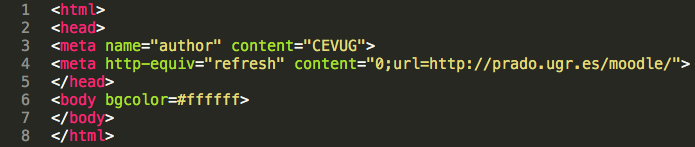
\includegraphics[width=1.0\textwidth]{../screenshots/redireccionhttp}
\caption{Redireccion HTTP al acceder a http://prado.ugr.es}
\label{redireccionhttp}
\end{figure}


Las versiones antiguas de moodle utilizaban la librería YUI desarrollada por Yahoo que fue declarada obsoleta el 29 de agosto de 2014 \cite{art_01} y a partir de la 2.9 se comenzó a migrar a la librería jQuery. Aunque moodle 2.6 utiliza YUI la plantilla Archaius usa varias funciones de la librería jQuery 1.10.2 \url{https://prado.ugr.es/moodle/theme/jquery.php/core/jquery-1.10.2.min.js} que fue liberada el 3 de Julio de 2013 y que teniendo en cuenta que la librería está ya por su versión 3.2 vemos que está claramente desactualizada.

Se está Apache como servidor HTTP, notar que se oculta su versión haciéndolo mas seguro ante posibles ataques dirigidos, esto es un acierto.

El servidor tiene instalada la versión 5.4.45 que fue liberada el 3 de septiembre de 2015 y que como podemos ver en \url{http://php.net/supported-versions.php} ya no está soportada. En este caso hay dos problemas, por un lado el usar una versión tan anticuada de PHP y por otra no ocultar la versión, siendo muy fácil encontrar vulnerabilidades para dicha versión.

\section{Entrevistas personales}

Como ya hemos comentado se hicieron una serie de entrevistas informales en las que simplemente se anotaban los puntos de vista de los usuarios así como sus quejas y sugerencias y se culminaba con un pequeño test de usabilidad consistente en pedir a los usuarios que cambiaran su foto de perfil de Prado2. En el test participaron cerca de 30 personas, tanto profesores y usuarios de Prado2 como gente externa que nunca había visto la plataforma.

Para cambiar la imagen de perfil de prado dos la ruta correcta a seguir es: Administración - > Editar Perfil - > Imagen del Usuario y aunque puede parecer sencillo nadie bajó del minuto y medio mientras probaba erráticamente en varios sitios, hubo un estudiante del Grado en Ingeniería Informática que tardó más de 4 minutos.

Todos los usuarios repetían básicamente el mismo patrón, como se les pedía que cambiaran la imagen del perfil lo primero que hacían era hacer click en la imagen para ver si salía alguna opción de editar, lo que deja entrever lo lejos que está la plantilla actual del uso real que hacen los usuarios. 

Además los distintos usuarios nos hicieron notar los siguientes problemas y/o carencias con los que se habían encontrado:

\begin{enumerate}


\item No te puedes desmatricular de asignaturas de otros cursos o de las que te has cambiado de grupo


\item Aunque se entre en inglés hay muchas cosas que aparecen en castellano, de hecho están mezclados ambos idiomas

\item La ventana de solicitud de contraseña de prado2 (el IDP del csirc) coge la configuración de idioma del navegador del usuario en lugar de la que viene de prado, esto hace que si por ejemplo tu navegador está en inglés pero tu estás mostrando prado en español, al acceder al IDP la ventana se mostrará en inglés.


\item Hay que bajar los materiales de la asignatura uno a uno en lugar de dar una opción para descargar todo el conjunto

\item Si se está navegando por la miga de pan se llegan a mostrar unos listados de asignaturas con mas de mil registro haciendo inusable el seleccionar alguna

\item El menú superior de asignaturas es inusable por los profesores pues no saben a ciencia cierta a que asignatura están accediendo hasta que han hecho click ya que muchas asignaturas comparten nombre simplemente cambiando los profesores

\item No se notifican los cambios y/o novedades en la plataforma, encontrando a veces que algo que funcionaba de una determinada manera ha cambiado, provocando confusión.

\item Si un alumno contiene un carácter no ascii como pueden ser vocales acentuadas o una "ñ", a la hora de descargar los trabajos de dicho alumno la codificación del archivo será incorrecta y al desempaquetar el archivo .zip en sistemas windows aparece una carpeta vacía (en sistemas Linux no hay problema). En este caso el profesor recibió una queja del alumno por que no le habían calificado una serie de ejercicios y el profesor estuvo haciendo comprobaciones en varios sistemas y lo puso en conocimiento del CSIRC, donde le aseguraron que era problema de su equipo. 

\item En determinados listados no aparecen barras de desplazamiento horizontal por lo que aparece la información cortada, en otros listados al contrario dichas barras son tan largas que en numerosas  ocasiones se ha perdido la localización espacial de la fila y se ha puntuado al alumno incorrecto.

\item Hay diferentes vistas de la ventana "Mis cursos" con la consecuente confusión

\item No se notifica a los usuarios cuando hay material nuevo o modificado obligando a comprobar periódicamente el material uno a uno.

\item Las calificaciones finales no se muestran aunque el profesor las publique.

\item A la hora de mostrar las calificaciones salen trozos de pruebas ocultas de otros cursos y otros grupos sin rellenar.

\item No se notifica la convocatorias de exámenes.

\item El sistema de mensajería es complicado de encontrar y mucho mas complicado de usar, primeramente el profesor ha de marcar uno a uno los alumnos no habiendo una opción para seleccionarlos todos, luego en lugar de aparecer un botón que ponga "Enviar mensaje" aparece un desplegable cuya única opción es "Enviar mensaje" (ver imagen \ref{fig:pantallazoPradoenviarMensaje}), al darle a esa opción pasamos a una ventana donde podemos redactar el mensaje aunque las opciones de insertar elementos no funcionan correctamente. En la parte inferior de ese mensaje vemos que aparece de nuevo toda la lista de alumnos sin respetar los que se habían marcado previamente. Al enviar el mensaje el profesor no recibe una copia pese a haberse marcado, con lo que no puede comprobar que efectivamente se está enviado el correo a todos los alumnos. El editor de mensajes no deja copiar/pegar con el botón derecho del ratón aunque si que deja hacerlo mediante atajos de teclado y por último y no menos importante no permite editar el asunto del mensaje. Si además sucede algún problema al enviar mensajes a los alumnos nos podemos encontrar con un críptico mensaje de error como el de la figura \ref{fig:pantallazoPradoMensaje2} que reza "Algo ha ido mal al enviar mensajes a los usuarios seleccioandos. Algunos pueden haber recibido el mensaje".


\begin{figure}[h!]
\centering
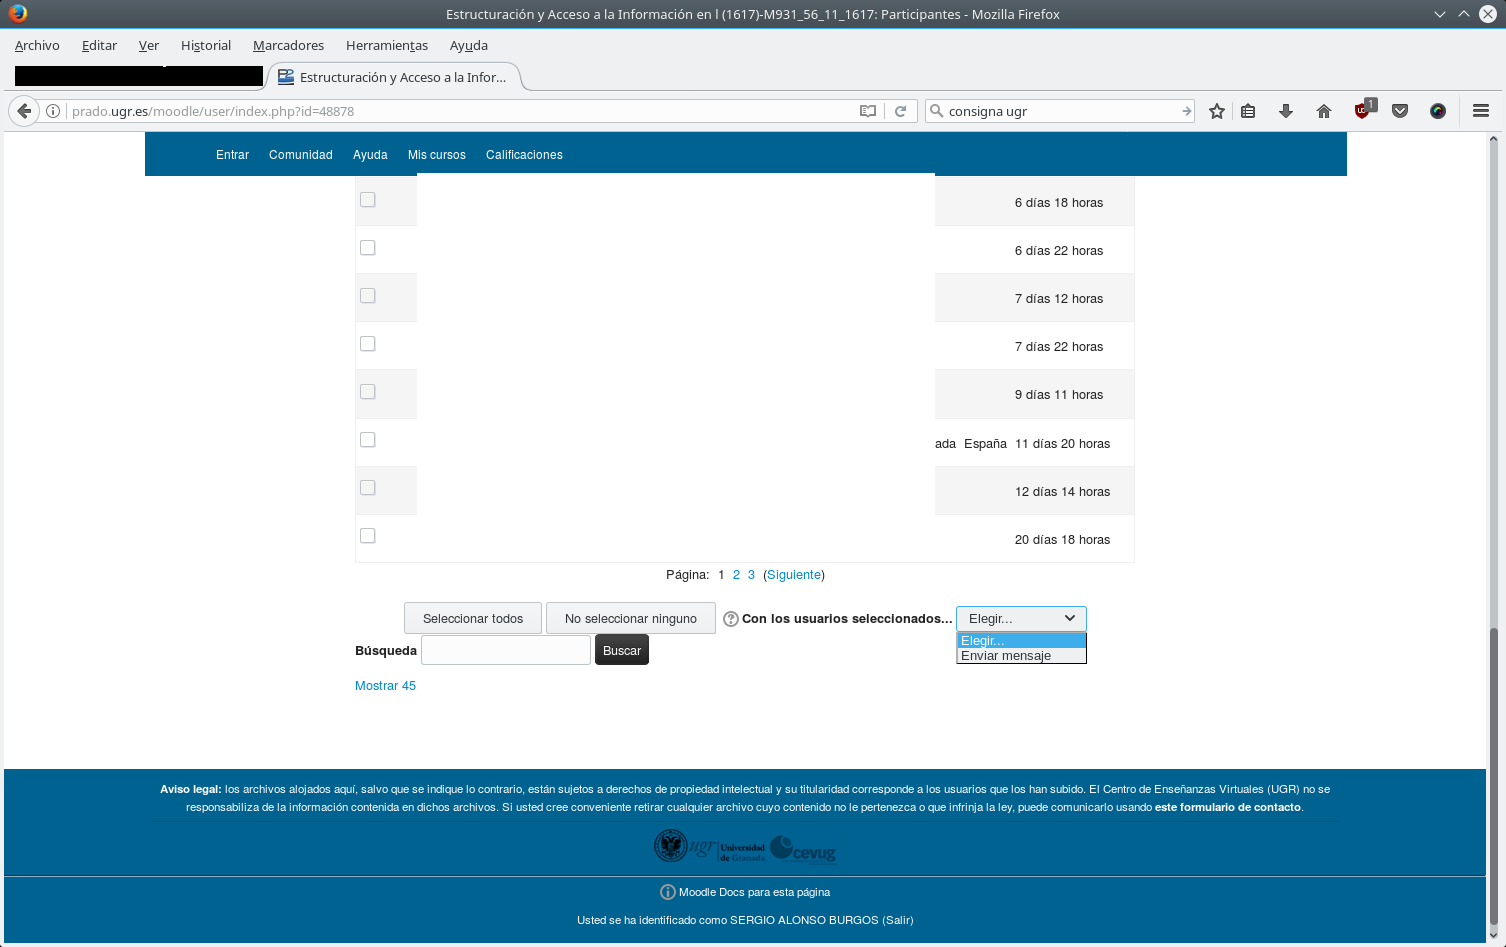
\includegraphics[width=0.8\textwidth]{../screenshots/pantallazoPradoenviarMensaje}
\caption{Vista principal del clon de Prado}
\label{fig:Lista desplegable Enviar Mensaje}
\end{figure}

\begin{figure}[h!]
\centering
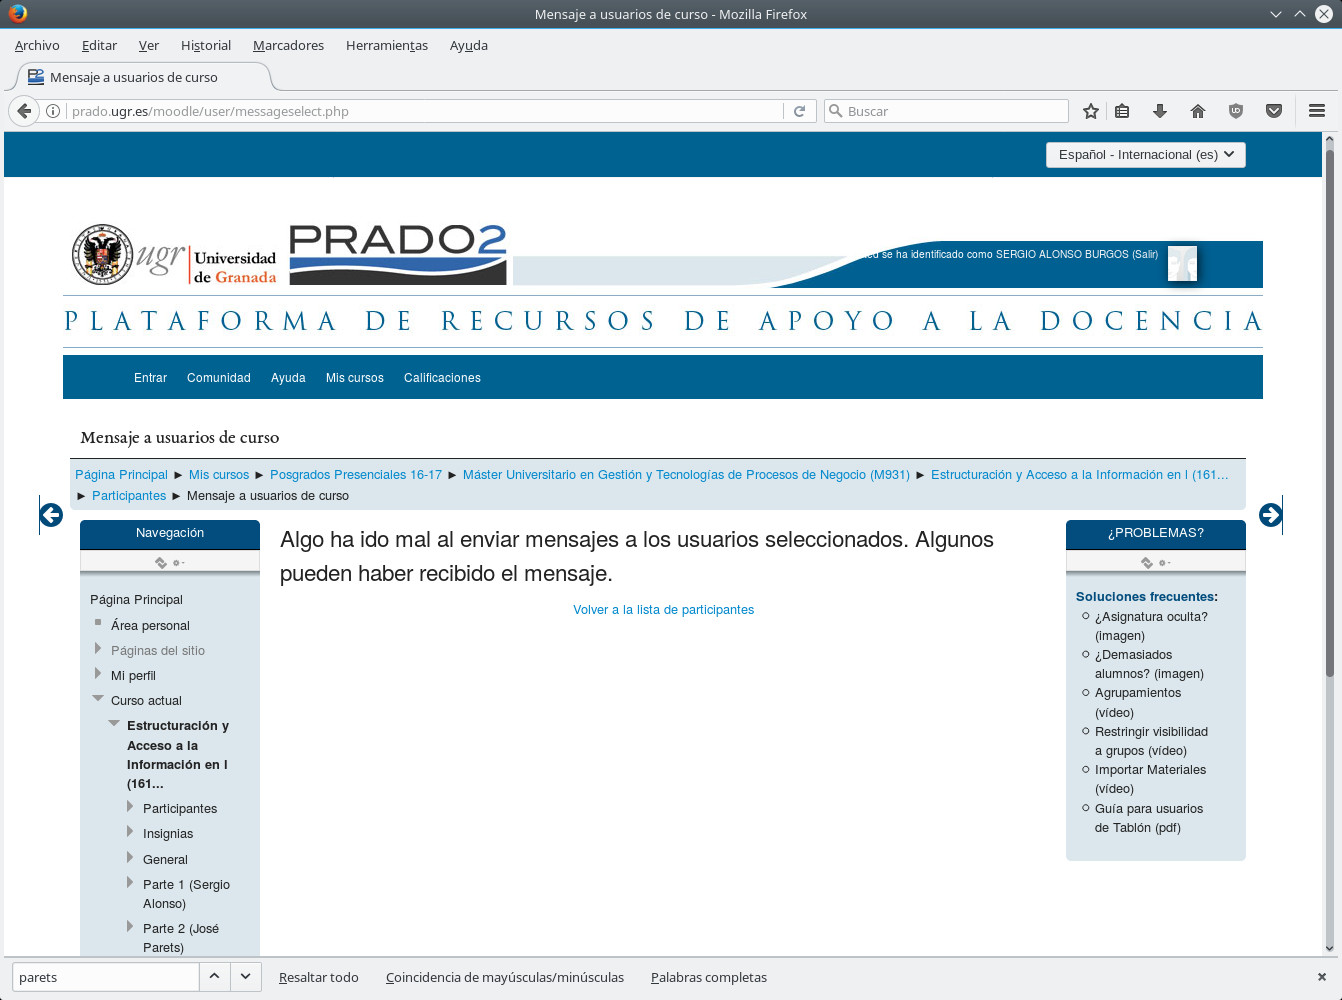
\includegraphics[width=0.8\textwidth]{../screenshots/pantallazoPradoMensaje2}
\caption{Error mostrado al enviar mensaje}
\label{fig:pantallazoPradoMensaje2}
\end{figure}


\item No hay una opción sencilla para crear un listado con los alumnos de cada grupo, opción que puede ser interesante, por ejemplo, para imprimir y llevar un control manual.

\item En la vista de grupos los nombres salen cortados y salen los apellidos de los alumnos pero no aparece el nombre, siendo un problema para alumnos con los mismos apellidos, además no se puede reordenar de ninguna forma.

\item El menú superior de Entrar, Comunidad, Ayuda, Mis cursos no tiene un sentido claro: La opción Entrar aparece siempre aunque la sesión esté iniciada, el menú Comunidad está accesible mas abajo y no tiene una importancia tal y como aparecer en ese menú, el menú Ayuda nos lleva a una pagina externa del CEVUG para abrir un ticket y el menú de cursos lleva a una vista que no es la misma que la de la página principal de Prado2.

\item La búsqueda de cursos suele tarda demasiado en responder.

\item Las novedades del curso y del sitio no parecen tener ninguna utilidad.

\item Aunque se configuren agrupamientos de alumnos, los mismos luego no se pueden utilizar para nada, de hecho no sirven ni para hacer un listado de alumnos por grupo.

\item No se entiende la utilidad del foro privado, quizá esa opción no debería estar, igual sucede con las insignias.

\item El árbol de navegación lateral es confuso y la estructura de bloques no es consistente, además en cada cambio de pagina se vuele a mostrar la vista por defecto, se puede hacer la prueba mostrando el bloque de calendario de la parte derecha haciendo click en cambiar de mes, vemos que se recarga la pagina ocultando de nuevo el bloque. Al entrar en la página aparecen a la izquierda 4 bloques diferenciados: Enlaces, Menú Principal, Navegación y Administración pero al entrar en cualquier opción los dos primeros desaparecen.

\item En los listados no se puede ordenar por rol del usuario, por lo que los distintos profesores de una asignatura aparecen mezclados con los alumnos.

\item Aunque se oculten los bloques laterales con las flechas que hay para tal cometido al recargar la página esos bloques vuelven a aparecer.


\item Si hago colapsar las columnas de navegación laterales (flechas izquierda y derecha), en cuanto pincho en otro enlace me vuelven a aparecer. Tengo que estar colapsándolas todo el rato y es un incordio.
\item En una ocasión probé a poner una práctica en la que había que usar el chat, pero los alumnos me dijeron que era muy poco funcional. Al parecer, costaba seguir una conversación, resultan preferibles los foros.
\item Las herramientas de grupos/agrupamientos me han dado algo de trabajo. Creo que ya lo controlo, pero me da la sensación de que podrían ser más fáciles.
\item Si envío un mensaje a un estudiante a través de moodle, no puedo poner un 'Asunto'. Imagino que simplemente le sale en 'Asunto' el nombre de la asignatura, pero me gustaría poder poner algo más específico.
\item Todos los cursos pongo un cuestionario de valoración de la asignatura que los estudiantes pueden responder anónimamente. Moodle preserva el anonimato en las respuestas, pero no en el 'registro de actividad'. Es decir, se puede saber quiénes respondieron al cuestionario e incluso, si uno estuviera muy pendiente de cada actualización de respuestas, quién es responsable de cada respuesta. Creo que cuando una actividad se etiqueta como anónima, el acceso a la misma debería desaparecer del registro de actividad.
\item Al poner una fecha de inicio y fin de una actividad, debería aparecer por defecto el año en que estamos. En una ocasión me ocurrió que la actividad se daba por cerrada un año antes.
\item No sé de quién depende esto pero, por favor, que aparezcan en moodle todos los estudiantes matriculados en la asignatura, y sólo ellos.

\item Es una locura el tema de la matrícula de los estudiantes; me han escrito estudiantes para decirme que a pesar de estar en otro curso y no haberse matriculado nunca en mi asignatura, aparecen y, por tanto, les llegan los mensajes y tienen acceso a la plataforma. Por el contrario, hay muchos estudiantes que tengo que matricular manualmente porque, a pesar de estar en mi grupo, no aparecen!!! 

\item El problema de la adjudicación de grupos de alumnos en el master de educación. Aparecen los alumnos de todas las especialidades en la misma asignatura y todos los profesores pueden subir o borrar recursos de la plataforma, aunque no sean profesores de ese grupo en concreto.



-Las sesiones de usuario (sobre todo cuando se visualiza desde el smartphone) se mantienen de una forma muy rara, ha habido veces que se ha cerrado sin motivo alguno y hay que volver a iniciar sesión. Adicionalmente, se debería habilitar un botón para recordar la sesión.
-La usabilidad deja mucho que desear, la plataforma no es nada intuitiva.
-En general los profesores no saben utilizar la opción de elegir grupo, optando por pasar una hoja en papel y que cada uno se apunte donde quiera.
-No se muestra con claridad los archivos nuevos o novedades en general, de forma que el usuario tiene que estar buscando qué ha visto ya y qué no.
-La plataforma funciona con lentitud y las caídas son muy frecuentes, en ocasiones en horas críticas para la entrega de ejercicios (entre las 22:00 y las 00:00)
-La plataforma en general carece de estilo y orden alguno, las cosas están por medio sin una estructura de calidad.

  Estaba haciendo unas cosas del Departamento y he tenido que acceder a Prado. Entonces he caído en la cuenta de otras dos cosas que no tenía anotadas y para las que no hay opción directa en Prado: poner el horario de teoría y prácticas de la asignatura y poner el horario de tutorías del profesorado implicado (tampoco sale en la parte personal). En general, los datos de la asignatura (incluso objetivos, temario de teoría y temario de prácticas) y los del profesorado que la imparte, brillan por su ausencia. Dos puntos más, y gordos, a favor de SWAD.

  Todas esas cosas las he podido poner en Prado, pero en un archivo en pdf que yo me he creado con la presentación de la asignatura.


\end{enumerate}

\section{Encuesta a los usuarios}

Durante el tiempo que estuvo operativa la encuesta recibimos un total de 617 respuestas, como se puede apreciar en el gráfico la mayor parte de las respuestas se obtuvieron tras las peticiones de participación via e-mail.

    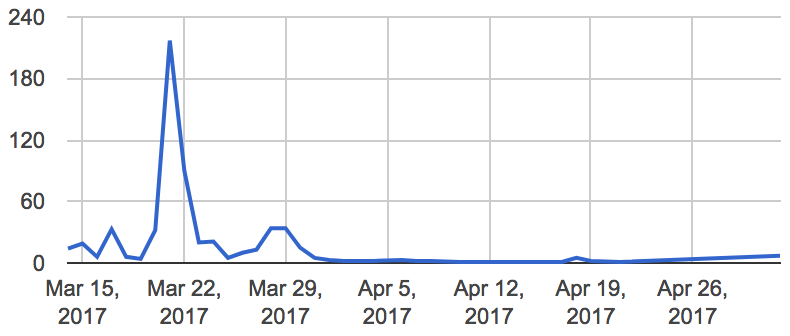
\includegraphics[width=0.8\textwidth]{../charts/00_fecha}
 	

\begin{enumerate}

  \item \textbf{Selección del tipo de usuario} 
  
  La mayor parte de los encuestados han sido alumnos superando el 83\% del ratio, casi un 15\% han sido profesores y el resto otro tipo de usuarios como pueden  ser estudiantes de doctorado y antiguos alumnos.
  
  
	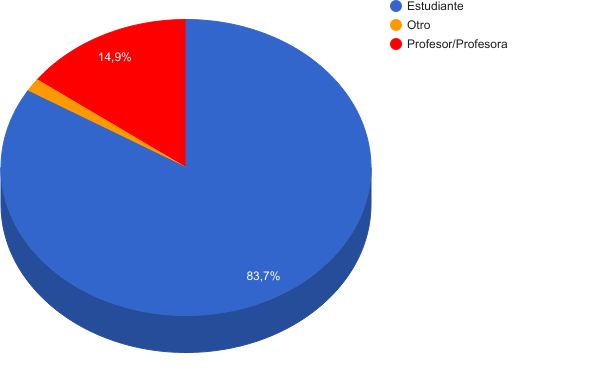
\includegraphics[width=0.8\textwidth]{../charts/01_esusted}
  

  \item \textbf{Selección de la titulación} 
  
  Debido al carácter de este proyecto esperábamos una mayoría de participantes de estudiantes de carreras impartidas en la ETSIIT como pueden ser el Grado de Ingeniería Informática, el Grado de Ingeniería en Tecnologías de Telecomunicación y el Doble Grado en Ingenierdía Informática y Matemáticas, pero nos ha sorprendido ver la alta participación de otros estudios como pueden ser Administración y Direccion de Empresas, Medicina y Psicología por nombrar las titulaciones mas representativos de las casi 70 participantes.
  
  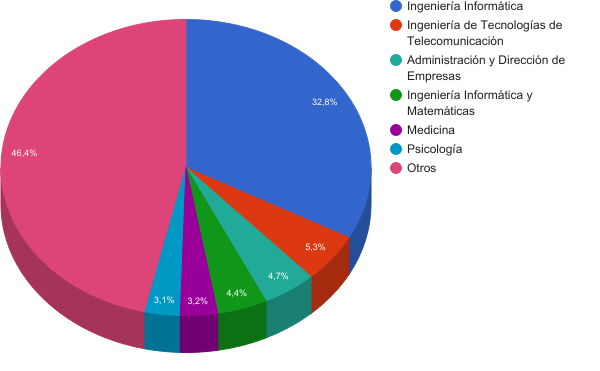
\includegraphics[width=0.8\textwidth]{../charts/02_titulacion}


  \item \textbf{¿Con qué periodicidad accede a Prado2?} 
  
  La mayoría de los usuarios acceden a la plataforma con mucha frecuencia lo que refuerza nuestra opinión de que por un lado se tiene que optimizar la plataforma para que esos accesos sean lo mas breves y satisfactorios posibles, muchos de estos accesos se reducirían si el sistema notificara via e-mail o via aplicación movil que hay novedades interesante en la plataforma. De igual manera se reduciría carga en el servidor si se supiera que los documentos subidos por el profesor no han subido cambios y no hubiera que descargarlos de nuevo para comprobarlo manualmente.

  
  
  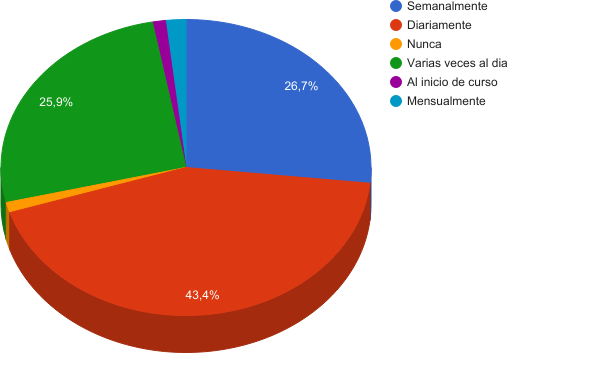
\includegraphics[width=0.8\textwidth]{../charts/03_periodicidad}

  
  \item \textbf{Califique las siguientes opciones según sus necesidades} 

Lo que mas piden los usuarios con diferencia es poder ver las calificaciones en Prado2, eso nos lo han hecho saber tanto en la opción de la encuesta como varios comentarios personales. Por otra parte muchos profesores nos han hecho saber que con el sistema actual tiene que hacer el trabajo por duplicado introduciendo las calificaciones en Prado2 y por otro lado en el sistema de actas de la UGR, cuando sería muchos mas cómodo poder generar en prado algún tipo de fichero CSV que les permitiera entregar las actas.

  
Casi todos los usuarios coinciden en que es vital el acceso desde dispositivos móviles, ya sea mediante una aplicación para smartphone como desde una web con un diseño adaptado a móviles ya que aunque el diseño actual tiene partes que si se adaptan para móviles no es apto para su uso ya que se hace inmanejable.

Los usuarios también creen necesario un sistema de mensajería interna para la comunicación entre profesores y alumnos.

En cambio, las opciones de Insignias, Blogs y Estadísticas no parecen ser vitales y de hecho mucha gente nos ha preguntado que utilidad tienen las Insginias pues no saben para que sirven.

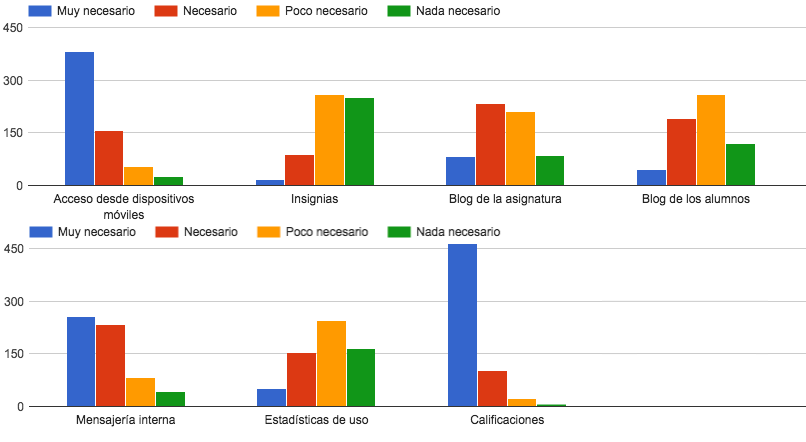
\includegraphics[width=0.8\textwidth]{../charts/04_califique} 

  \item \textbf{Actividades y recursos} 

En cuanto a actividades podemos ver que al igual que en las instalaciones de moodle de otras universidades las opciones mas usadas son las de agregar tareas y archivos, hay que tener en cuenta que hay actividades que básicamente son similares a agregar archivo, como puede ser carpeta, documento, página y libro. 

Aunque moodle tiene actividades que podrían ser muy útiles, como pueden ser los paquetes SCORM e IMS, el desconocimiento y/o la falta de formación hace que la gente ignore para que sirven.

Igual pasa con algunas tareas espécificas creadas para la UGR como pueden ser las clases grabadas (GA3), aunque si hay tareas que son necesarias aunque tengan muy poca utilización como pueden ser la selección de grupo de prácticas al inicio del curso y el control de asistencia.


\begin{figure}[H]
\centering
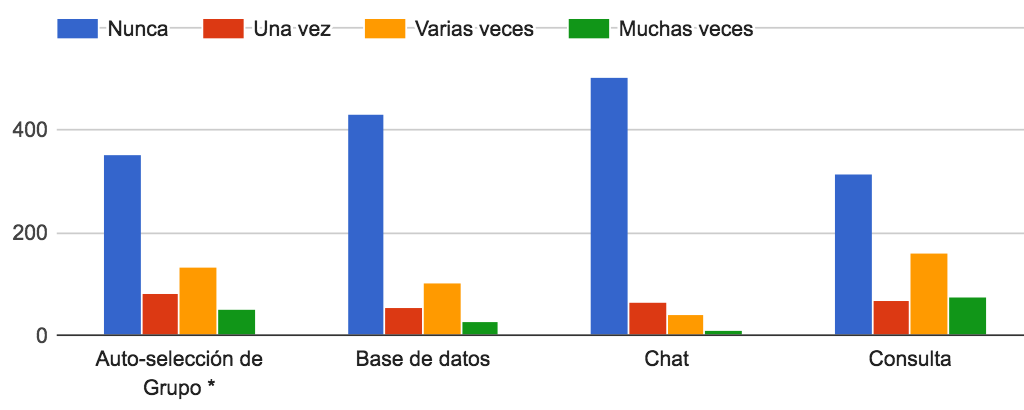
\includegraphics[width=0.8\textwidth]{../charts/05_actividades_01} 
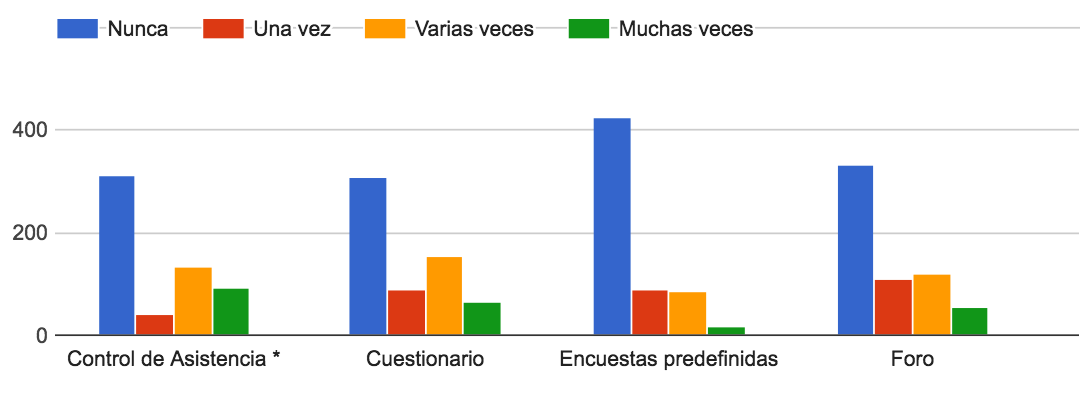
\includegraphics[width=0.8\textwidth]{../charts/05_actividades_02} 
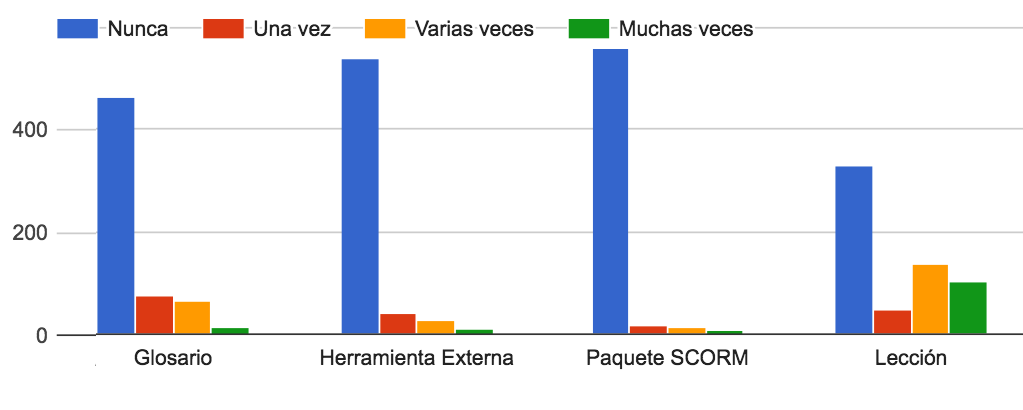
\includegraphics[width=0.8\textwidth]{../charts/05_actividades_03} 
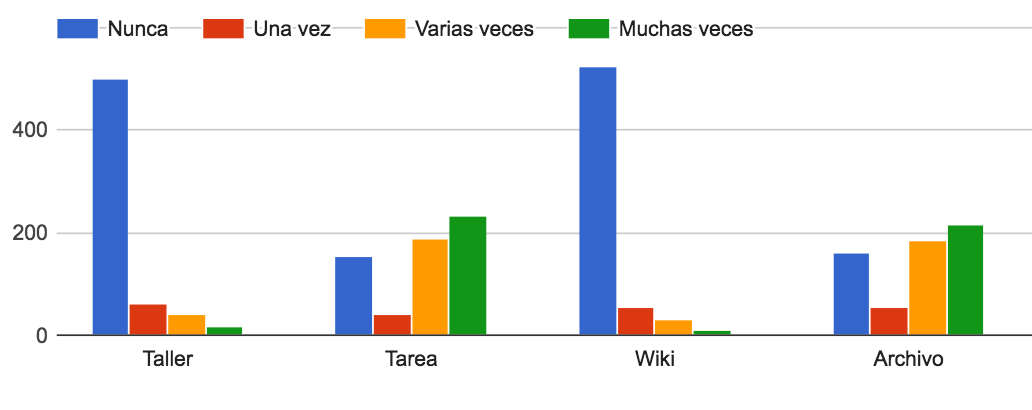
\includegraphics[width=0.8\textwidth]{../charts/05_actividades_04} 
\end{figure}
\begin{figure}[H]
\centering
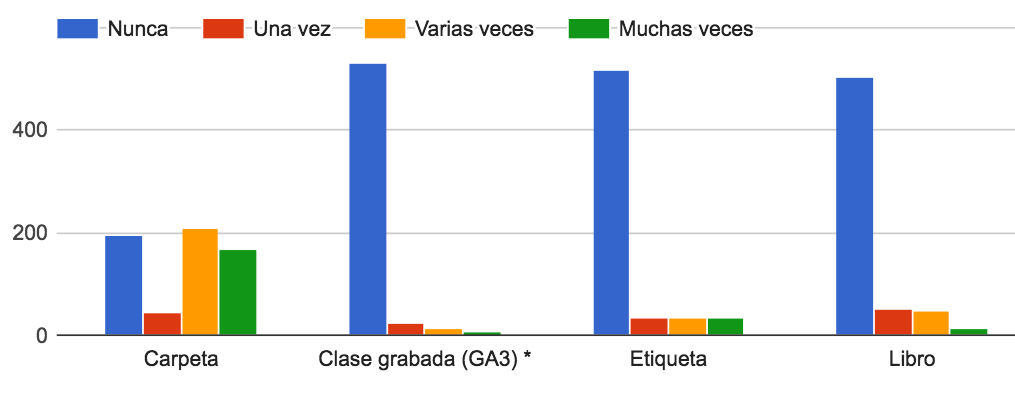
\includegraphics[width=0.8\textwidth]{../charts/05_actividades_05} 
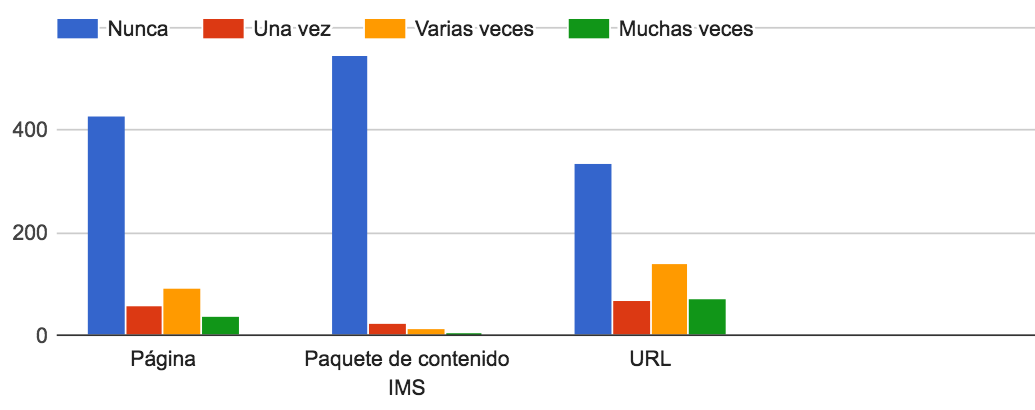
\includegraphics[width=0.8\textwidth]{../charts/05_actividades_06} 

\end{figure}






  \item \textbf{¿Cómo calificaría Prado2?}
  
  
A la hora de calificar prado han la mayoría de los usuarios han otorgado aprobado lo cual es una buena señal, aunque se piense que hay un descontento generalizado la gente entiende que una plataforma puede tener problemas y simplemente espera que se solucionen. Aun con el aprobado general, los usuarios si que encuentran en gran medida muy deficiente la usabilidad de la plataforma. En cambio el sentimiento general es el de que la plataforma es segura.

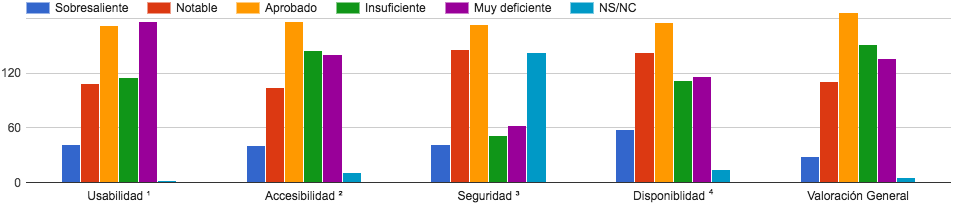
\includegraphics[width=0.8\textwidth]{../charts/06_calificaria}


  \item \textbf{¿Con cúales de las siguientes plataformas de la UGR ha trabajado?} 

Aquí hay tres ganadores claves, y son evidentemente las plataformas que mas se han usado en todo el ámbito UGR como pueden ser el Tablon de Docencia, SWAD y el propio Prado2, luego encontramos plataformas usadas solo en la ETSIIT como pueden ser Tutor y DECSAI y algunos otros como el antiguo moodle del CEVUG y Ágora que es otra instalación de moodle utilizada en la facultad de Psicología.

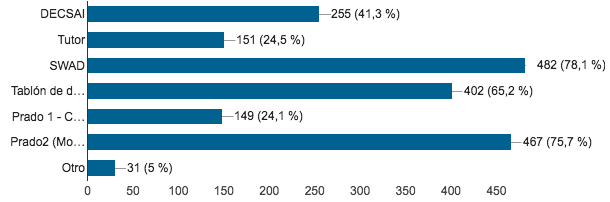
\includegraphics[width=0.8\textwidth]{../charts/07_plataformastrabajado}

  \item \textbf{De las siguientes plataformas de la UGR ¿Cuál prefiere?} 

A la hora de establecer la plataforma favorita está clara la prevalencia de SWAD ya que es una plataforma potente y con muchos años de uso aunque Prado2 también tiene una buena acogida y mas teniendo en cuenta la sensación de descontento generalizado que percibíamos antes de comenzar este proyecto, esto quiere decir que tampoco se va por mal camino con la plataforma actual. Curioso cuanto menos que el Tablón de Docencia, una arcaica plataforma utilizada en la UGR sigue teniendo sus partidarios pero como ya hemos comentado anteriormente una de las cosas con las que más cuesta lidiar en cuanto a la usabilidad es la resistencia de los usuarios al cambio, aunque este sea a mejor.

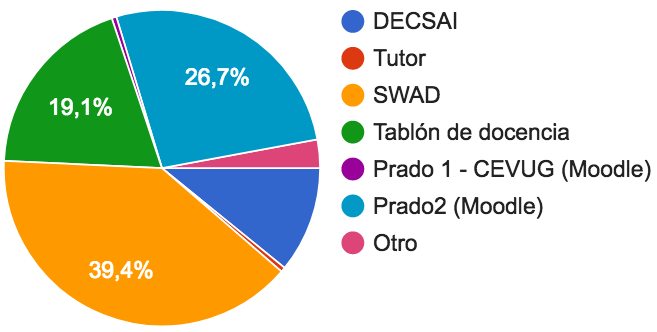
\includegraphics[width=0.8\textwidth]{../charts/08_plataformas_prefiere} 

  \item \textbf{¿Ha encontrado algún error que debería ser subsanado en Prado2?} 

Esta pregunta al ser de entrada libre se adjuntará en el listado en bruto de respuestas   

  \item \textbf{Indique cuál es la funcionalidad que más le gusta de Prado2} 

Esta pregunta al ser de entrada libre se adjuntará en el listado en bruto de respuestas

  \item \textbf{Comentarios adicionales} 
  
Esta pregunta al ser de entrada libre se adjuntará en el anexo VI
  
\end{enumerate}


\section{Análisis de registros propios de la plataforma}

Tras analizar los registros proporcionados por el CEVUG de los años 2015 y 2016 vemos que los resultados de la encuesta cuadran con los mismos.

No hemos analizado la muestra que nos proporcionaron de 2014 ya que fue en el curso 2015-2016 como se puede apreciar en la figura \ref{fig:distintonumerousuarios_2015}.

Lo primero a destacar son el notable incremento de peticiones del año 2015 al año 2016 que se puede apreciar en la tabla de la figura \ref{table:sumarioregistros}.

\begin{table}[H]
\centering
\begin{tabular}{|l|r|r|}
\hline
\textbf{Año}        & \textbf{2015}	& \textbf{2016} \\ \hline
Número de registros & 3.119.094     	& FALTA				\\ \hline
Usuarios únicos     & 19.448        & FALTA				\\ \hline
IPs distintas       & 115.349       & FALTA				\\ \hline
Cursos              & 1.266         & FALTA				\\ \hline
Módulos             & 32            & FALTA				\\ \hline
\end{tabular}
\caption{Sumario de los registros de los años 2015 y 2016}
\label{table:sumarioregistros}
\end{table}

En las figuras de la \ref{fig:actividadtotal_2015} a la \ref{fig:frecuenciausuarios_2015} podemos ver como el grueso de la actividad se lo llevan unos pocos usuarios, es decir, la inmensa mayoría interactúa muy poco con la plataforma. Presuponemos que este grueso de actividad pertenece tanto a los administradores como a un reducido círculo de profesores, hay que tener en cuenta que los logs registran cada click en alguna sección de Prado.

\begin{figure}[H]
\centering
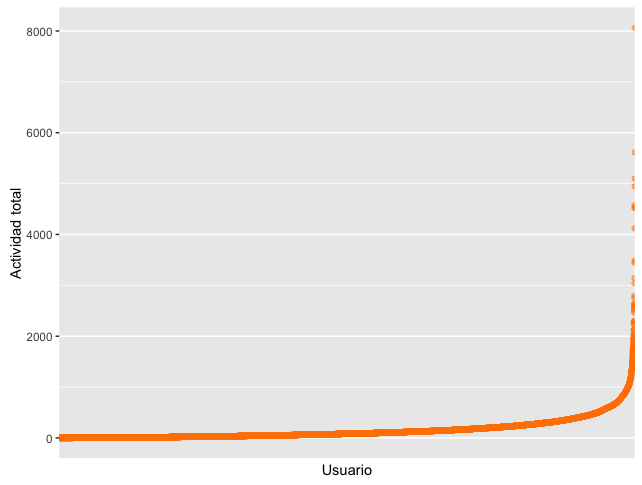
\includegraphics[width=0.9\textwidth]{../r/actividadtotal_2015}
\caption{Actividad total en 2015}
\label{fig:actividadtotal_2015}
\end{figure}

\begin{figure}[H]
\centering
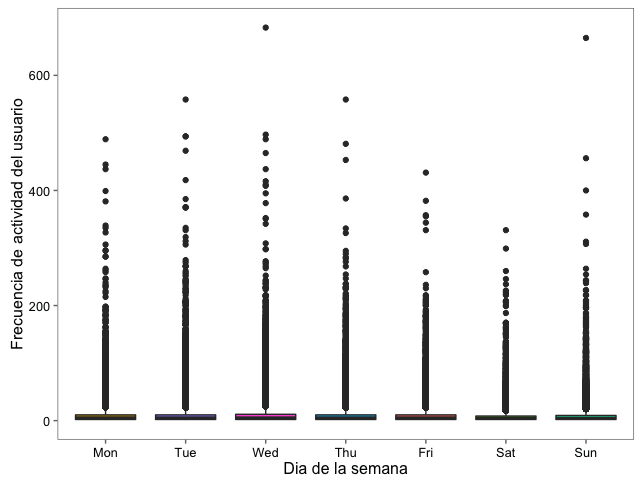
\includegraphics[width=0.9\textwidth]{../r/frecuenciaactividadusuario_2015}
\caption{frecuenciaactividadusuario}
\label{fig:frecuenciaactividadusuario_2015}
\end{figure}

\begin{figure}[H]
\centering
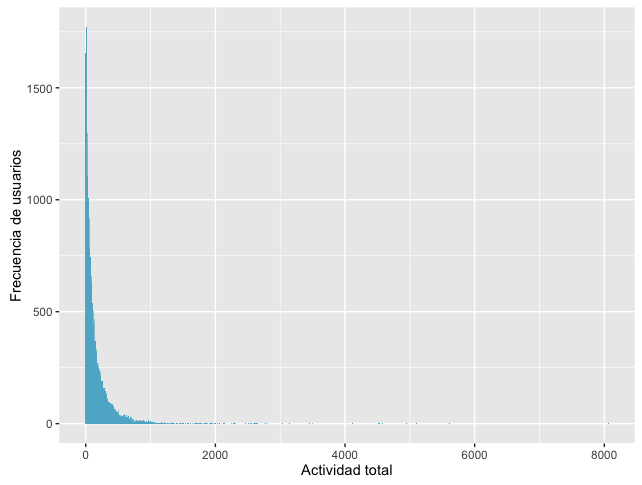
\includegraphics[width=0.9\textwidth]{../r/frecuenciausuarios_2015}
\caption{frecuenciausuarios}
\label{fig:frecuenciausuarios_2015}
\end{figure}

También vemos en las figuras \ref{fig:distintonumerousuarios_2015} y FALTA como los usuarios comenzaron a hacer uso de la plataforma en Septiembre de 2015 que es cuando oficialmente se comenzó a utilizar Prado.



\begin{figure}[H]
\centering
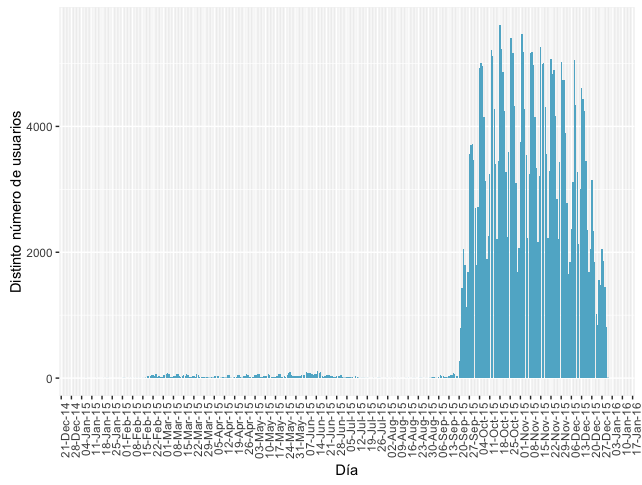
\includegraphics[width=0.9\textwidth]{../r/distintonumerousuarios_2015}
\caption{Interacciones de usuarios únicos en 2015}
\label{fig:distintonumerousuarios_2015}
\end{figure}

En las figuras \ref{fig:frecuenciaactividaddiaria_2015} y FALTA se percibe como la mayoría de los usuarios utilizan la plataforma en las horas lectivas, descenciendo la utilización como es evidente los fines de semana, también nos sirve para ver como la madrugada es la hora ideal para realizar cambios en la plataforma pues el a esas horas casi no hay usuarios usando Prado.

\begin{figure}[H]
\centering
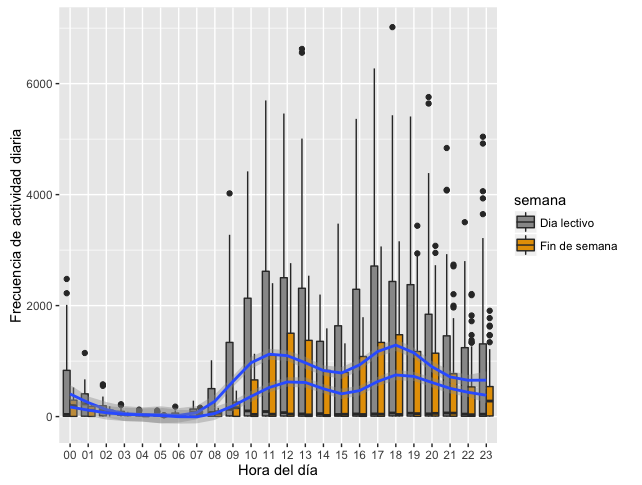
\includegraphics[width=0.9\textwidth]{../r/frecuenciaactividaddiaria_2015}
\caption{Frecuencia de actividad diaria en 2015}
\label{fig:frecuenciaactividaddiaria_2015}
\end{figure}


En cuanto a las actividades podemos ver en las figuras \ref{fig:usoactividades_2015} y FALTA así como en la tabla \ref{table:usoactividades_2015} que tal y como concluimos en la encuesta la gran mayoría de las actividades disponibles en moodle no tienen apenas uso. Hay que destacar que la actividad 'course' se refiere a cada vez que un usuario ve contenido de un curso acaparando la mitad de las interacciones y que la actividad 'user' se crea cada vez que se ve el perfil de un usuario o profesor. Exceptuando estos dos casos vemos como las mas usados los cuestionarios y los archivos.

\begin{figure}[H]
\centering
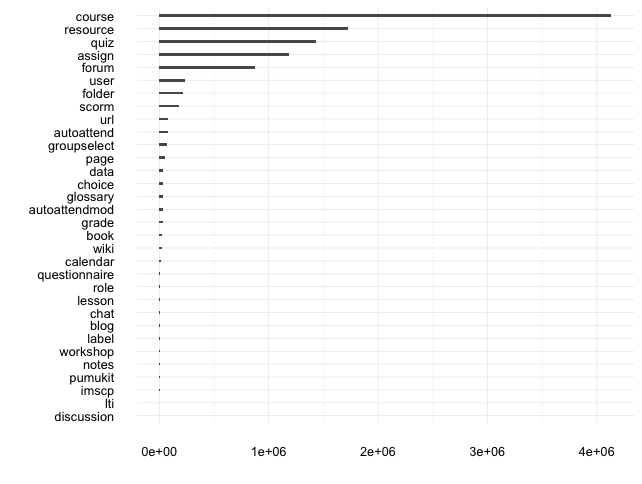
\includegraphics[width=0.9\textwidth]{../r/usoactividades_2015}
\caption{usoactividades}
\label{fig:usoactividades_2015}
\end{figure}

\begin{table}[H]
\centering
\begin{tabular}{|l|r|r|}
\hline
\textbf{Módulo} & \textbf{2015} & \textbf{2016} \\ \hline
course          & 1204043       & FALTA         \\ \hline
quiz            & 480975        & FALTA         \\ \hline
resource        & 464898        & FALTA         \\ \hline
assign          & 381096        & FALTA         \\ \hline
forum           & 233528        & FALTA         \\ \hline
user            & 81118         & FALTA         \\ \hline
folder          & 65733         & FALTA         \\ \hline
scorm           & 33459         & FALTA         \\ \hline
url             & 25720         & FALTA         \\ \hline
autoattend      & 25530         & FALTA         \\ \hline
groupselect     & 25518         & FALTA         \\ \hline
page            & 22382         & FALTA         \\ \hline
choice          & 11514         & FALTA         \\ \hline
autoattendmod   & 11020         & FALTA         \\ \hline
glossary        & 9244          & FALTA         \\ \hline
lesson          & 6702          & FALTA         \\ \hline
wiki            & 6040          & FALTA         \\ \hline
calendar        & 4988          & FALTA         \\ \hline
questionnaire   & 4961          & FALTA         \\ \hline
data            & 4525          & FALTA         \\ \hline
book            & 4485          & FALTA         \\ \hline
grade           & 2809          & FALTA         \\ \hline
role            & 2306          & FALTA         \\ \hline
blog            & 1665          & FALTA         \\ \hline
chat            & 1351          & FALTA         \\ \hline
label           & 1282          & FALTA         \\ \hline
notes           & 1174          & FALTA         \\ \hline
imscp           & 396           & FALTA         \\ \hline
pumukit         & 305           & FALTA         \\ \hline
discussion      & 118           & FALTA         \\ \hline
workshop        & 117           & FALTA         \\ \hline
lti             & 92            & FALTA         \\ \hline
\end{tabular}
\caption{Tabla detallada del uso de actividades en 2015 y 2016}
\label{table:usoactividades_2015}
\end{table}




\section{Análisis de usabilidad de la plataforma}

Para el análisis de usabilidad he hecho uso de las directrices vistas en los libros de Jakob Nielsen \cite{jakonielsen} y de Tania Schlatter \cite{taniaschlatter} y basándome también en mi experiencia como desarrollador web.

Lo primero que llama la atención al entrar en la plataforma es el banner central de información que acapara toda la atención obligando al usuario a desplazarse para ver la información de los cursos que quiere ver.

Pienso que una plataforma va a ser usada en su mayor medida por alumnos y profesores quizá se debería dar prioridad a la información de los cursos en lugar de información superflua, así encontrarían la información de manera mas rápida aumentando su grado de satisfacción

El tener varias vistas de las mismas secciones da lugar a confusión, por ejemplo la vista principal muestra los cursos en los que estoy matriculado y si hago click en la vis muestra la misma información con algunas diferencias pero es una vista distinta de cuando le doy a la opción 

\section{Análisis de accesibilidad de la plataforma}

En cuanto al análisis de accesibilidad, 



Aplicacion movil


\section{Análisis de seguridad}



\begin{verbatim}

MOODLEID1_ cookie

ngrep



sudo ngrep -q "^GET .* HTTP/1.[01] "host prado.ugr.es"

MOODLEID1_


sudo tcpdump -I -i en0 -s 0 -B 524288 -w eduroam.pcap

sudo ngrep -q "^GET .* HTTP/1.[01].*MOODLEID1_=" "host prado.ugr.es" -I eduroam.pcap


arp spoofing



sudo ettercap -T -i en0 -P autoadd -M arp ///80 -e "^GET /moodle/ HTTP/1.[01].*MOODLEID1_=" -t tcp


curl -v --cookie " MoodleSession=1k3arpnhojmnjh0rv3ckuee7m2; MOODLEID1%25AB%25FE%2589%25D2O%25D7%2513; SimpleSAMLSessionID-sp=c77c96971496cb79b0f2d5b0ead74452; SimpleSAMLAuthToken=_07cd74595444d3f665543a8af7ebb20b16e7352e94;" http://prado.ugr.es/moodle/

\url{https://es.wikipedia.org/wiki/ARP_Spoofing}

\url{http://insecure.org/sploits/arp.games.html}

title="Ver perfil">ERNESTO SERRANO COLLADO</a>

Todo software se desarrolla para cubrir una necesidad, por lo que en este apartado vamos a describir los requisitos que se estiman necesarios para cubrir los objetivos propuestos.

\url{https://github.com/TUM-MZ/moodle-block_material-download}

fijarse en estas encuestas

\url{http://stackoverflow.com/insights/survey/2017/ }



sobre https
\url{http://www.elladodelmal.com/2017/04/presto-parking-un-sitio-web-pci.html}


corregidas vulnerabilidades en moodle
\url{http://unaaldia.hispasec.com/2017/04/corregidas-cuatro-vulnerabilidades-en.html}

\end{verbatim}





\section{Análisis de disponibilidad}

Como ya hemos indicado anteriormente el 30 de enero de 2017 comenzamos a monitorizar la disponibilidad de Prado2 con la herramienta StatusCake. Como podemos ver en los periodos de disponiblidad de la figura \ref{fig:statuscake1} es una web que realmente goza de una buena disponibilidad por periodos de hasta incluso 40 días. Aunque podemos ver algunos tramos en los que la página no está accesible, estos periodos suelen ser de una duración razonable y a unas horas en las que no se espera que haya demasiados usuarios utilizando la plataforma.

\begin{figure}[h!]
\centering
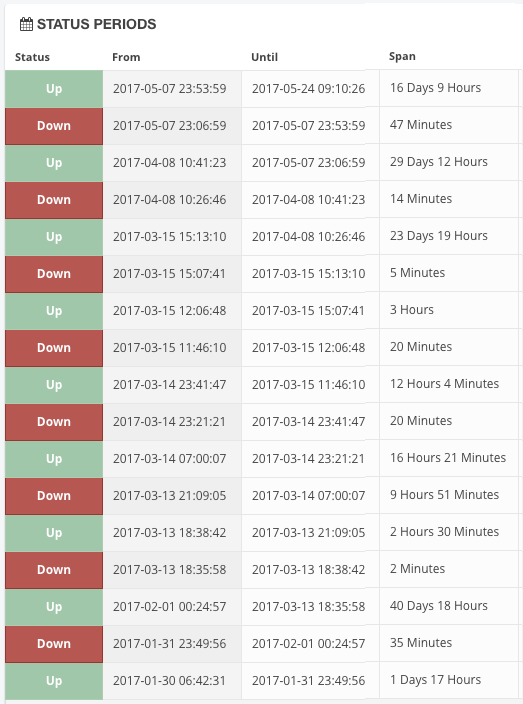
\includegraphics[width=0.8\textwidth]{../screenshots/statuscake1}
\caption{Disponibilidad medida por StatusCake}
\label{fig:statuscake1}
\end{figure}

Pero vemos como el 13 de marzo de 2017 hubo algún tipo de problema que se tardó bastante en solucionar y que mantuvo la plataforma sin acceso mostrando un mensaje (ver figura \ref{fig:pradocaido}) que tampoco daba a los usuarios demasiada información del problema. El mayor problema de esta caída fue el desconocimiento de los usuarios de qué estaba pasando.

\begin{figure}[h!]
\centering
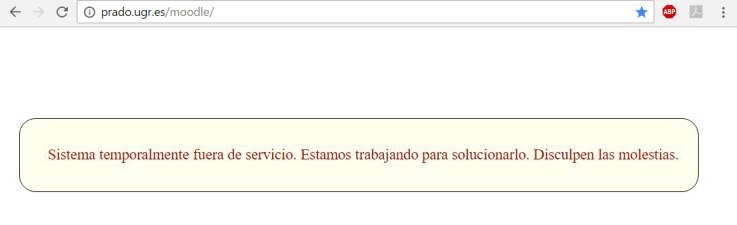
\includegraphics[width=0.8\textwidth]{../images/pradocaido}
\caption{Mensaje de error mostrado por Prado2}
\label{fig:pradocaido}
\end{figure}



Lo ideal en un servicio con tanto volumen de usuarios y tan crítico es informar a los usuarios de posibles cortes en el servicio. Por ejemplo, SWAD suele avisar con una notificación a todos los usuarios de futuros cortes del servicio (ver imagen \ref{fig:paroprogramadoswad}), ya que aunque el servicio se suspenda de madrugada al tener tantos usuarios siempre puede afectar a una gran parte de ellos. 

\begin{figure}[h!]
\centering
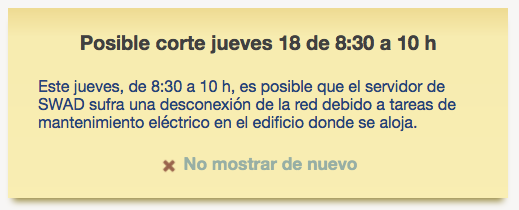
\includegraphics[width=0.8\textwidth]{../images/paroprogramadoswad}
\caption{Aviso de parada programada en SWAD}
\label{fig:paroprogramadoswad}
\end{figure}

En el caso de no poder preveer un problema de de este tipo es recomendable al menos avisar a los usuarios por una vía alternativa como puede ser el correo institucional o las redes sociales. En el caso de la caída de Prado del día 13  de marzo aunque mucha gente alertaba en la red social Twitter de que tenían problemas para acceder a la plataforma no se recibió ninguna respuesta de la UGR hasta el restablecimiento del servicio como podemos ver en la imagen \ref{fig:tweet}. 



\begin{figure}[h!]
\centering

\includegraphics[width=0.8\textwidth]{../images/tweet}
\caption{Tweet avisando del restablecimiento del servicio}
\label{fig:tweet}
\end{figure}

Como podemos ver en la imagen \ref{fig:statuscake2} el tiempo de respuesta del servidor es bastante bueno, ya que aunque lo ideal suelen ser 200 milisegundos en cargar la página principal Prado2 suele responder en un rango que va dsde los 400 milisegundos, que está muy bien, a los 3 segundos, que se puede considerar dentro de lo aceptable. Quizá reseñar que en caso de alta demanda como puede ser el inicio del curso puede ser interesante contar con sistema de balanceo de carga para evitar los problemas que nos han comentado algunos usuarios que se han encontrado a la hora de registrarse en un grupo de prácticas, ya que al haber tanta gente conectada al mismo tiempo el sistema se ha visto colapsado. 



\begin{figure}[H]
\centering
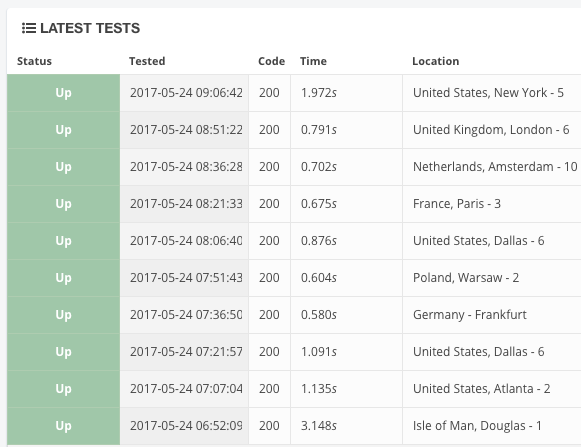
\includegraphics[width=0.8\textwidth]{../screenshots/statuscake2}
\caption{Tiempo de respuesta medido por StatusCake}
\label{fig:statuscake2}
\end{figure}


\section{Clonado de la plataforma}

Se creó el subdominio \url{http://prado.ernesto.es} en mi servidor personal y se instaló la versión 2.6.4 de moodle, luego se procedió a instalar el tema Archaius  (ver imagen \ref{fig:archaius} y a copiarle los estilos CSS en el fichero /theme/archaius/style/custom.css, copiar la imagen de cabecera (ver imagen \ref{fig:cabeceraprado} y en un tiempo mínimo teníamos funcionando un sistema casi idéntico al prado original (ver imagen \ref{fig:pradoernesto} donde agregamos unas cuantas asignaturas así como alumnos y profesores para probar las distintas opciones de moodle.

\begin{figure}[H]
\centering

\includegraphics[width=0.8\textwidth]{../screenshots/cabeceraprado}
\caption{Imagen cabecera de Prado}
\label{fig:cabeceraprado}
\end{figure}

\begin{figure}[H]
\centering
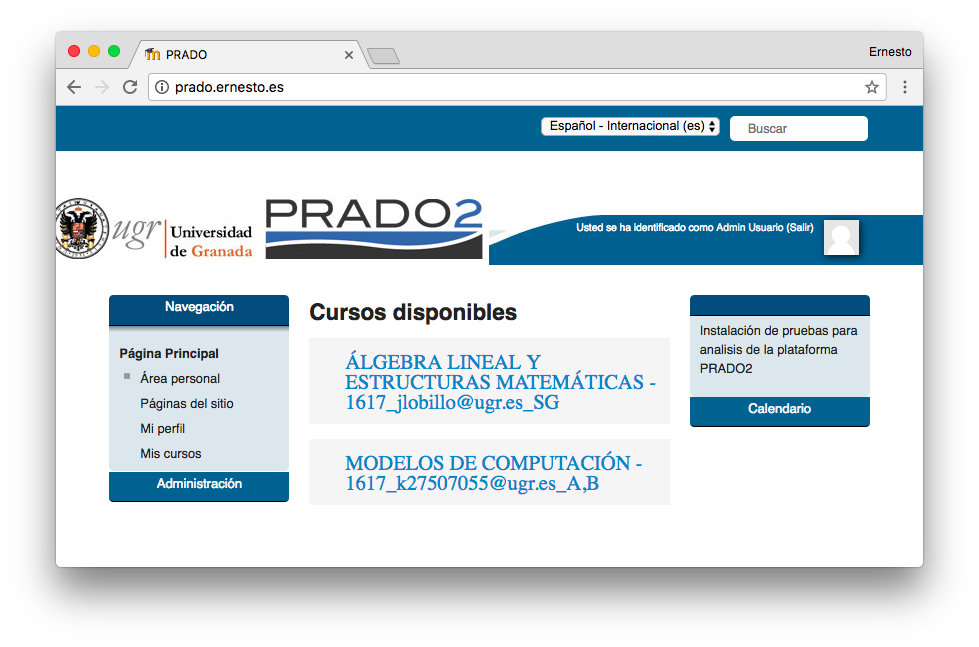
\includegraphics[width=0.8\textwidth]{../screenshots/pradoernesto}
\caption{Vista principal del clon de Prado}
\label{fig:pradoernesto}
\end{figure}

\begin{figure}[H]
\centering
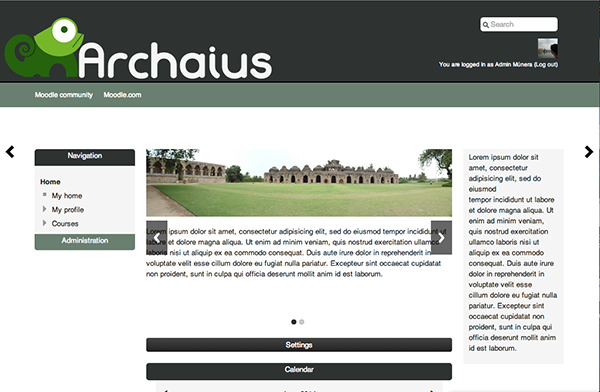
\includegraphics[width=0.8\textwidth]{../screenshots/archaius}
\caption{Captura del tema Archaius sin modificaciones}
\label{fig:archaius}
\end{figure}




\section{Realización de script GreaseMonkey}

Cuando comenzamos el proyecto pensamos en el desarrollo de una herramienta que corrigiera algunas de las carencias mas importantes de la plataforma. 
Como ya habíamos comprobado previamente la página no se mostraba correctamente por https porque habían rutas absolutas a elementos http y el navegador las bloqueaba por considerarlas inseguras pero si cambiábamos las urls de esos elementos la página se visualizaba correctamente.
Para ello escribimos un código que buscaba todas las urls que comenzaran por http y las reemplazaba por https haciendo uso de expresiones regulares. Este código funcionaba correctamente pero al hacer los cambios una vez cargada daba una sensación extraña y mucha sensación de lentitud. Aparte de esto hicimos varias pruebas y vimos que aunque la página se recargara sobre https el servidor de identificación de sesión del a ugr (\url{https://idp.ugr.es/simplesaml/module.php/core/loginuserpass.php} devolvía los valores a una página http, por lo que siempre se podían capturar los valores devueltos aunque el resto de la sesión fuera sobre un canal seguro. 

Además, pudimos comprobar que haciendo unos cambios mínimos en nuestro clon propio de la plataforma esta se devolvía siempre de forma correcta por https sin tener que recurrir a parches externos y siendo una mejor solución.

Por hacer una ultima prueba quisimos probar si sería posible hacer cambios estéticos en la plataforma por lo que inyectamos el código \texttt{\$( '.block' ).css( 'display' , 'block' );} que simplemente le dice mediante javascript que despliegue todos los bloques laterales de la página lo cual hacía que la navegación fuese un poco menos caótica pero al igual que lo anterior sin llegar a ser una solución del todo viable y limitándose a un simple parche temporal así que finalmente descartamos el desarrollo del script, de todas formas hemos considerado incluir lo desarrollado en los anexos.


\section{Herramienta hardware para robo de sesiones}

Para desarrollar la herramienta utilizamos un viejo router Huawei HG556a de Vodafone al que le instalamos el firmware libre OpenWRT \cite{openwrt}. 

Una vez instalado el firmware configuramos dos interfaces inalámbricas virtuales. La primera intefaz se configuró en modo cliente que conectamos a la red \textit{eduroam} haciendo uso de los certificados pertinentes y mi cuenta personal de usuario de la UGR. La segunda interfaz se configuró en modo punto de acceso, creando una red wifi sin contraseña de nombre \textit{eduroam\_pruebas} y agregamos las reglas necesarias a iptables para que redirigiera el trafico de una interfaz a otra por lo que los clientes que se conectaban a la red wifi \textit{eduroam\_pruebas} realmente estaban saliendo a internet por la red \textit{eduroam} pero con la salvedad de que podíamos espiar el tráfico que pasaba por la red. A este tipo de dispositivos de les denomina \textit{honeypot} (tarro de miel). 

Instalamos el programa \textit{ettercap} que utilizamos durante la auditoría de seguridad y lo configuramos para empezar a capturar información. A los pocos minutos de empezar a capturar nos dimos cuenta que el limitado espacio del dispositivo iba a ser un problema, pues el HG556a cuenta con sólo 16MB de ROM y 64MB de RAM a todas luces insuficiente para una captura de este tipo así que conectamos una unidad USB de 16GB, la montamos como lectura/escritura y solucionamos el problema del espacio. 

Una vez vimos que el sistema funcionaba probando a secuestrar nuestras sesiones fuimos a la sala de libre acceso que hay al lado de la biblioteca de la ETSIIT en la que habían unos 15 estudiantes, conectamos el aparato, lo disimulamos entre unas mochilas y volvimos a comprobar que todo funcionaba correctamente y podiamos capturar nuestras variables de sesión si nos conectábamos a prado a través de esta red. 

Hicimos un poco de ingeniería social comentando en voz alta que estaban probando una nueva red wifi que se llamaba \textit{eduroam\_pruebas} que iba mucho más rápida y nos pusimos a esperar. En dos horas que estuvimos en la sala contabilizamos un total de 37 clientes conectados al router, de los cuales 18 se conectaron a prado y de todos ellos pudimos capturar sus variables de sesión. 

Evidentemente aunque vimos los valores de las variables de sesión en ningún momento hicimos uso de ellas para suplantar la identidad de nadie, ya que no contábamos con la autorización debida, todo fue un ejercicio confirmar nuestras sospechas de que era realmente fácil realizar un ataque a la plataforma.




